
\documentclass{exam}

\usepackage{units} 
\usepackage{graphicx}
\usepackage[fleqn]{amsmath}
\usepackage{cancel}
\usepackage{float}
\usepackage{mdwlist}
\usepackage{booktabs}
\usepackage{cancel}
\usepackage{polynom}
\usepackage{caption}
\usepackage{fullpage}
\usepackage{xfrac}
\usepackage{enumerate}

\newcommand{\degree}{\ensuremath{^\circ}} 
\everymath{\displaystyle}

% \begin{figure}[H]
%   \centering
%   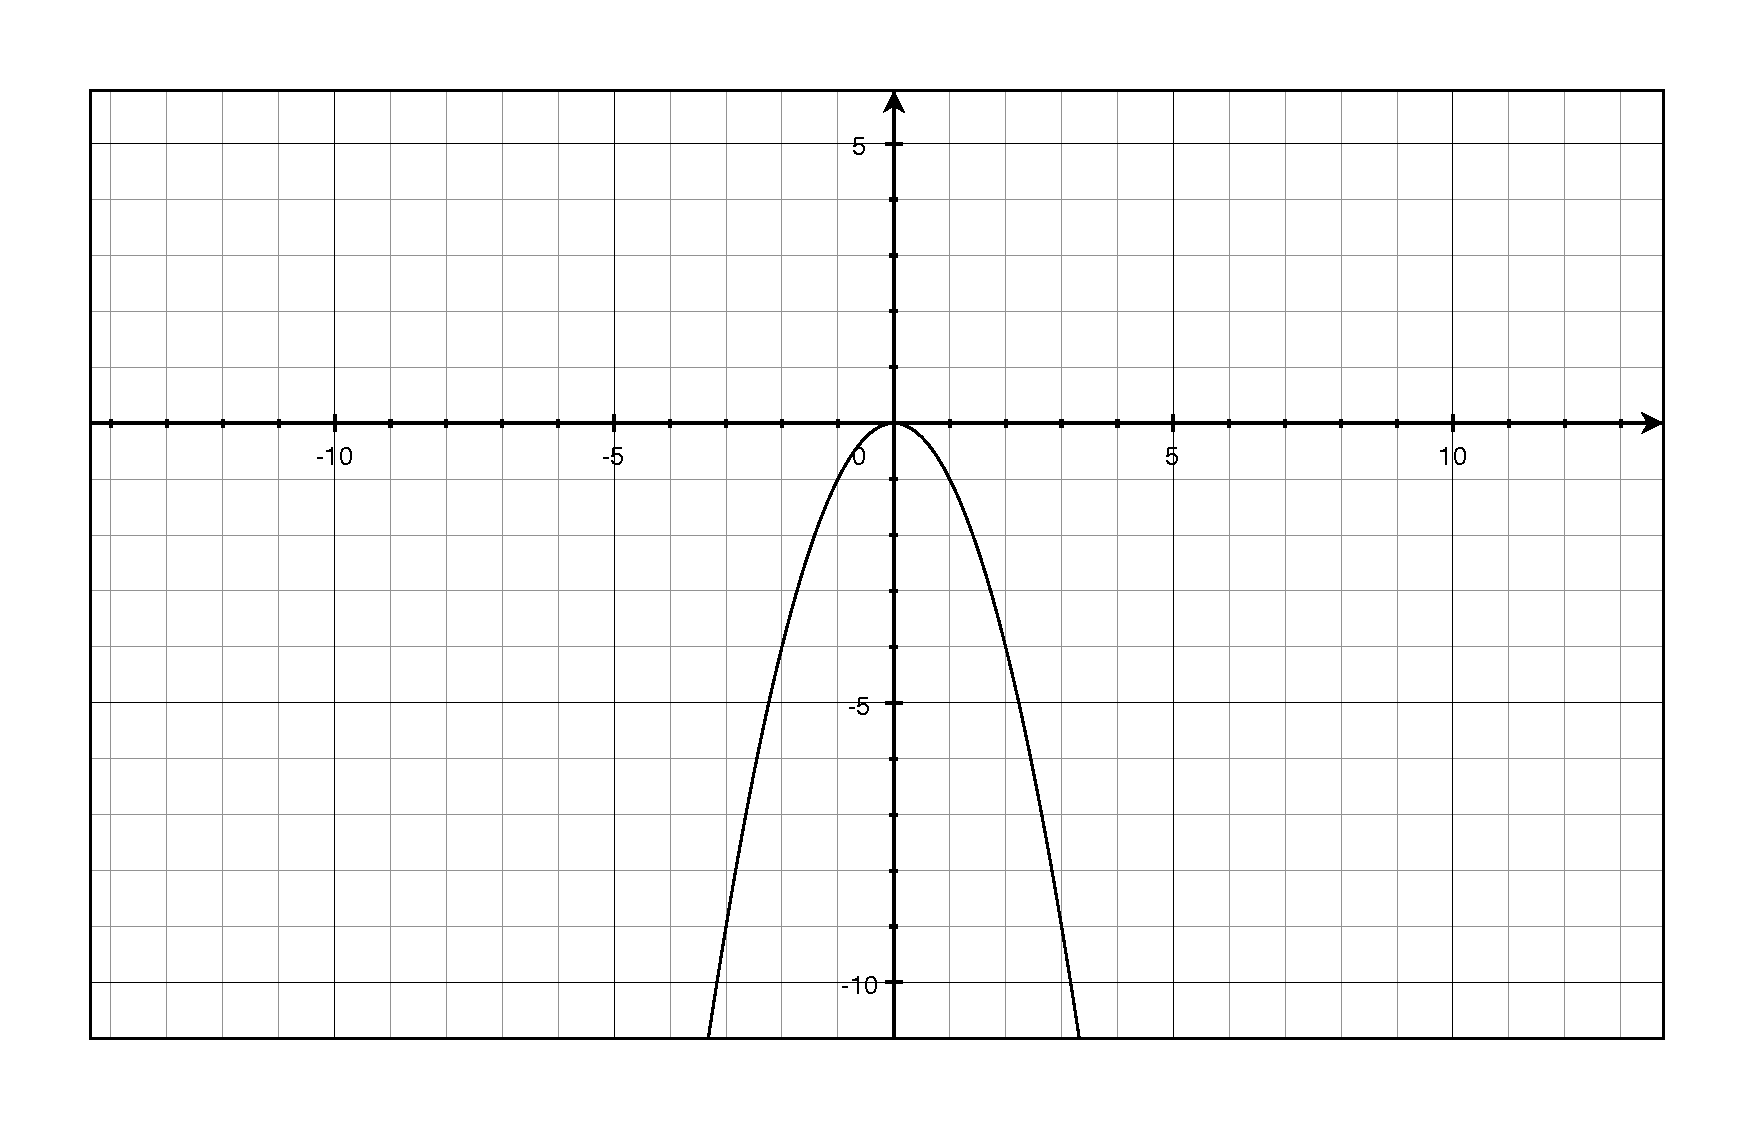
\includegraphics[scale=0.9]{problem7.eps}
%   \caption*{Problem 7}
% \end{figure}

% \begin{tabular}{cc}
%   \toprule
%   period & amplitude \\
%   \midrule
%   value one & value two
%   \bottomrule
% \end{tabular}

\printanswers

\ifprintanswers 
  \usepackage{2in1, lscape} 
\fi

\date{June 5, 2013}
\author{}
\title{Math 141 \\ Homework 13}

\begin{document}

  \maketitle

  \section{Homework}

  Section 4.2: 

  \section{Extra Credit}
  Section 4.2, TO DO

  \ifprintanswers
    \begin{description}
      \item[49] TO DO
    \end{description}

  \section{Review}

  \begin{enumerate}
    \item Simplify: $\frac{\sqrt{-4}\sqrt{-27}\sqrt{-16}}{\sqrt{-3}}$
      \begin{solution}
        \begin{align*}
          \frac{\sqrt{-4}\sqrt{-27}\sqrt{-16}}{\sqrt{-3}} &= \frac{2i \cdot 3i \sqrt{3} \cdot 4i}{i \sqrt{3}} \\
          &= \frac{24i^3 \sqrt{3}}{i \sqrt{3}} \\
          &= 24 i^2 \\
          &= -24 \\
        \end{align*}
      \end{solution}

  \end{enumerate}
    \section{Section 4.2}

    \begin{description}

      \item[3] 
        \begin{align*}
          5^2 &= 25 \\
          5^0 &= 1 \\
        \end{align*}

    \item[4] 
      \begin{align*}
        10^{-1} &= 0.1 \\
        8^3 &= 512 \\
      \end{align*}

    \item[5] 
      \begin{align*}
        8^{1/3} &= 2 \\
        2^{-3}  &= \frac{1}{8} \\
      \end{align*}

    \item[6] 
      \begin{align*}
        4^5     &= 81 \\
        8^{2/3} &= 4 \\
      \end{align*}

    \item[7] 
      \begin{align*}
        e^x &= 5 \\
        e^5 &= y \\
      \end{align*}

    \item[8] 
      \begin{align*}
        e^2 &= x + 1 \\
        e^4 &= x - 1 \\
      \end{align*}

    \item[9] 
      \begin{align*}
        \log_5 125       &= 3 \\
        \log_{10} 0.0001 &= -4 \\
      \end{align*}

    \item[10] 
      \begin{align*}
        \log_{10} 1,000 &= 3 \\
        \log_{81} 9     &= \frac{1}{2} \\
      \end{align*}

    \item[11] 
      \begin{align*}
        \log_{8} \frac{1}{8} &= -1 \\
        \log_{2} \frac{1}{8} &= -3 \\
      \end{align*}

    \item[12] 
      \begin{align*}
        \log_{4} 0.125 &= - \frac{3}{2} \\
        \log_{7} 343   &= 3 \\
      \end{align*}

    \item[13] 
      \begin{align*}
        \ln 2 &= x \\
        \ln y &= 3 \\
      \end{align*}

    \item[14] 
      \begin{align*}
        \ln 0.5 &= x + 1 \\
        \ln t &= 0.5x \\
      \end{align*}

    \item[15]
      \begin{align*}
        \log_3 3   &= 1 \\
        \log_3 1   &= 0 \\
        \log_3 3^2 &= 2 \\
      \end{align*}

    \item[16]
      \begin{align*}
        \log_5 5^4 &= 4 \\
        \log_4 64  &= 3 \\
        \log_9 9   &= 1 \\
      \end{align*}

    \item[17]
      \begin{align*}
        \log_6 36     &= 2 \\
        \log_9 81     &= 2 \\
        \log_7 7^{10} &= 10 \\
      \end{align*}

    \item[18]
      \begin{align*}
        \log_2 32     &= 5 \\
        \log_8 8^{17} &= 17 \\
        \log_6 1      &= 0 \\
      \end{align*}

    \item[19]
      \begin{align*}
        \log_3 \left( \frac{1}{27} \right) &= -3 \\
        \log_{10} \sqrt{10}                &= \frac{1}{2} \\
        \log_5 0.2                         &= \log_5 \left( \frac{2}{10} \right) \\
                                           &= \log_5 \left( \frac{1}{5} \right) \\
                                           &= -1 \\
      \end{align*}

    \item[20]
      \begin{align*}
        \log_5 125      &= 3 \\
        \log_{49} 7     &= \frac{1}{2} \\
        \log_9 \sqrt{3} &= \log_9 3^{1/2} \\
                        &= \log_9 9^{1/4} \\
                        &= \frac{1}{4} \\
      \end{align*}

    \item[21]
      \begin{align*}
        2^{\log_2 37}    &= 37 \\
        3^{\log_3 8}     &= 8 \\
        e^{\ln \sqrt{5}} &= \sqrt{5} \\
      \end{align*}

    \item[22]
      \begin{align*}
        e^{\ln \pi}  &= \pi \\
        10^{\log 5}  &= 5 \\
        10^{\log 87} &= 87 \\
      \end{align*}

    \item[23]
      \begin{align*}
        \log_{8} 0.25 &= \log_8 \left( \frac{1}{4} \right) \\
                      &= \log_8 2^{-2} \\
                      &= \log_8 {2^3}^{-2/3} \\
                      &= - \frac{2}{3} \\
        \\
        \ln e^4 &= 4 \\
        \\
        \ln \left( \frac{1}{e} \right) &= \ln e^{-1} \\
                                       &= -1 \\
      \end{align*}

    \item[24]
      \begin{align*}
        \log_4 \sqrt{2} &= \log_4 2^{1/2} \\
                        &= \log_4 4^{1/4} \\
                        &= \frac{1}{4} \\
        \\
        \log_4 \left( \frac{1}{2} \right) &= \log_4 \left( \frac{1}{4^{1/2}} \right) \\
                                          &= \log_4 4^{-1/2} \\
                                          &= - \frac{1}{2} \\
        \\
        \log_4 8 &= \log_4 2^3 \\
                 &= \log_4 \left[ 4^{1/2} \right]^3 \\
                 &= \log_4 4^{3/2} \\
                 &= \frac{3}{2} \\
      \end{align*}

    \item[25]
      \begin{enumerate}[a]
        \item 
          \begin{align*}
            \log_2 x     &= 5 \\
            2^{\log_2 x} &= 2^5 \\
            x            &= 32 \\
          \end{align*}

        \item 
          \begin{align*}
            \log_2 16     &= x \\
            x &= 4 \\
          \end{align*}
      \end{enumerate}

    \item[26]
      \begin{enumerate}[a]
        \item 
          \begin{align*}
            \log_5 x     &= 4 \\
            5^{\log_5 x} &= 5^4 \\
            x            &= 625 \\
          \end{align*}

        \item 
          \begin{align*}
            \log_{10} 0.1 &= x \\
            x &= -1 \\
          \end{align*}
      \end{enumerate}

    \item[27]
      \begin{enumerate}[a]
        \item 
          \begin{align*}
            \log_3 243 &= x \\
            x &= 5 \\
          \end{align*}

        \item 
          \begin{align*}
            \log_3 x     &= 3 \\
            3^{\log_3 x} &= 3^3 \\
            x            &= 27 \\
          \end{align*}
      \end{enumerate}

    \item[28]
      \begin{enumerate}[a]
        \item 
          \begin{align*}
            \log_4 2 &= x \\
            x        &= \log_4 4^{1/2} \\
                     &= \frac{1}{2} \\
          \end{align*}

        \item 
          \begin{align*}
            \log_4 x     &= 2 \\
            4^{\log_4 x} &= 4^2 \\
            x            &= 16 \\
          \end{align*}
      \end{enumerate}

    \item[29]
      \begin{enumerate}[a]
        \item 
          \begin{align*}
            \log_{10} x      &= 2 \\
            10^{\log_{10} x} &= 10^2 \\
            x                &= 100 \\
          \end{align*}

        \item 
          \begin{align*}
            \log_{5} x     &= 2 \\
            5^{\log_{5} x} &= 5^2 \\
            x              &= 25 \\
          \end{align*}

      \end{enumerate}

    \item[29]
      \begin{enumerate}[a]
        \item 
          \begin{align*}
            \log_x 1000     &= 3 \\
            x^{\log_x 1000} &= x^3 \\
            x^3             &= 1000 \\
            x               &= 10 \\
          \end{align*}

        \item 
          \begin{align*}
            \log_x 25     &= 2 \\
            x^{\log_x 25} &= x^2 \\
            x^2           &= 25 \\
            x             &= 5 \\
          \end{align*}
      \end{enumerate}


    \end{description}

  \else
    \vspace{6 cm}
    \begin{quote}
      \begin{em}
        TO DO
      \end{em}
    \end{quote}

    \hspace{1 cm} --Henry David Thoreau
  \fi

\end{document}

